\documentclass[a4paper, oneside]{csthesis}

\usepackage{etex}
\reserveinserts{28}

% package to be able to use special characters
\usepackage[utf8]{inputenc}

% Sophisticated math package
\usepackage{amsmath}

% Special symbols
\usepackage{amssymb}

\usepackage{siunitx}

% nicely render theorems and proofs
\usepackage[standard,thmmarks,amsmath]{ntheorem}

\usepackage{graphicx}

% package to format pseudo-code. Check the package documentation.
% http://ctan.org/pkg/listings
\usepackage{algorithmic}
\usepackage{algorithm}

% awesome code highlighting and coloring for many languages
% http://en.wikibooks.org/wiki/LaTeX/Packages/Listings
\usepackage{listings}
\lstset{language=Java}

% Provides \xspace command that evaluates to a space if the next character in the source is a blank and
% no space if next character is no blank. Useful in command definitions.
\usepackage{xspace}

% Provides a more flexible tabular environment
\usepackage{tabularx}

% Enables the use of the H location specifier for float environments that puts the float exactly where it is located in the source.
\usepackage{float}

% Enables the use of colours
\usepackage{color}

\usepackage{paralist}

% nice string commands
\usepackage{xstring}

\usepackage{colortbl}
\usepackage[table]{xcolor}

% wide tables
\usepackage{adjustbox}

\definecolor{DarkGray}{gray}{0.7}
\definecolor{MiddleGray}{gray}{0.8}
\definecolor{Gray}{gray}{0.9}

\definecolor{darkblue}{rgb}{0,0,.5}
% Enables clickable links in the PDF and additional PDF specific configuration options.
\usepackage[
            colorlinks=true,
            linkcolor=darkblue, urlcolor=darkblue, citecolor=darkblue,
						raiselinks=true,
            bookmarks=true,
            bookmarksopenlevel=1,
            bookmarksopen=true,
            bookmarksnumbered=true,
            hyperindex=true,
            plainpages=false,
            pdfpagelabels=true,
            pdfstartview=FitH,
            pdfstartpage=1,
            pdfpagelayout=OneColumn
            ]{hyperref}

% Provides a highly configurable way to create references inside the document and automatically prefix
% the number reference by fig./eq./chapter and so on. You only have to use \cref{label} or \Cref{label}
% to obtain "Lemma 4.1" or "Corollary 4.1" etc., depending on the label. See an example in the proof
% of the first theorem or check the documentation of the package for further information.
\usepackage[noabbrev]{cleveref}


% awesome figure placment
\usepackage{subfigure}

% Load own command definitions, a few helpful ones are already defined there.

% This alters the numbering of theorems and lemmas.
\theoremsymbol{\ensuremath{\scriptstyle \Diamond}}
\renewtheorem{theorem}{Theorem}[chapter]
\renewtheorem{lemma}[theorem]{Lemma}
\renewtheorem{corollary}[theorem]{Corollary}
\renewtheorem{definition}[theorem]{Definition}

% This creates a two new theorem-like environments
\theoremsymbol{}
\newtheorem{notation}[theorem]{Notation}
\theorembodyfont{}
\newtheorem*{problem}{Problem}

\crefname{algorithm}{algorithm}{algorithms}
\Crefname{algorithm}{Algorithm}{Algorithms}

% This changes the comment style of the "algorithmic" pseudocode package
\renewcommand\algorithmiccomment[1]{\hfill \small \(\triangleright\) #1}

% This creates four commands to leave annotations in your document
\newcommand{\TODO}[1]{\noindent {{\color{red}\fbox{\sffamily \bfseries TODO}} \sffamily #1}}
\newcommand{\FIXME}[1]{\noindent {{\color{green}\fbox{\sffamily \bfseries FIXME}} \sffamily #1}}
\newcommand{\CONSIDER}[1]{\noindent {{\color{blue}\fbox{\sffamily \bfseries CONSIDER}} \sffamily #1}}
\newcommand{\RW}[1]{\noindent \color{blue}#1}

% This creates a command to easily refer to websites as footnotes
\newcommand{\websource}[3]{\footnote{{#1\newline Available at: #2 [Accessed
#3]}}}

\newcommand\telesto{\textit{Telesto}}

\graphicspath{{figures/}}

% style whole rows in table
\usepackage{array}
\newcolumntype{$}{>{\global\let\currentrowstyle\relax}}
\newcolumntype{^}{>{\currentrowstyle}}
\newcommand{\rowstyle}[1]{\gdef\currentrowstyle{#1}%
  #1\ignorespaces
}


%%%%%%%%%%%%%%%%%%%%%%%%%%%%%%%%%%%%%%%%%%%%%%%%%%%%%%%%%%%%%%%%%%%%%%%%%%%%%%%%%%%%%%%%%%%%%%%%%
% DOCUMENT METADATA

\thesistype{Report Group 32}
\title{Analytical Queuing Model for Telesto}

\author{Dominic Langenegger}
\email{dominicl@student.ethz.ch}
\institute{Advanced Systems Lab 2013 \\[2pt]
Systems Group \\[2pt]
ETH Z\"urich}

% You can put in your own logo here "\includegraphics{...}" or just comment the command
% \logo{}

\supervisors{Markus Pilman\\[2pt] Prof.\ Dr.\ Gustavo Alonso}

% You can comment the following two commands if you don't need them
\keywords{}
%\categories{ACM categories go here.}

\date{December 20, 2013}

%%%%%%%%%%%%%%%%%%%%%%%%%%%%%%%%%%%%%%%%%%%%%%%%%%%%%%%%%%%%%%%%%%%%%%%%%%%%%%%%%%%%%%%%%%%%%%%%%

\begin{document}

\frontmatter
\maketitle % do not remove this line

\cleardoublepage

%\begin{acknowledgements}
%\end{acknowledgements}


\begin{abstract}
	This report summarizes the work of analytically modeling and evaluating
	\telesto, the Distributed Message Passing System built by Simon Marti and
	Dominic Langenegger during the first milestone of the course project of the
    {\it Advanced Systems Lab} course 2013 at ETH Zurich. All relevant
    information about the first milestone can be found in \cite{asl:telesto}.

    Used concepts, mathematical formulas and theoretical aspects are heavily
    based on \cite{jain2008art} and the lecture slides.
    
\end{abstract}

\tableofcontents

\mainmatter % do not remove this line

% Start writing here
\chapter{Introduction}
    

\chapter{Analytical Queuing Model}
    This chapter introduces the analytical queuing model built to model the
    characteristics of \telesto. It also includes explanations about
    simplifications and assumptions that were made.

    We recall Table 5.3 in \cite{asl:telesto}, showing in which parts of the
    system a request spends how much time:
    
    \begin{table}[hp]
        \centering
        \rowcolors{1}{Gray}{white}
        \begin{tabular}{$l^c^r}
            \rowcolor{DarkGray}
            \rowstyle{\bfseries}
            Phase & Time & Relative\\
            \hline
            Waiting for client & \SI{79}{\micro\second} & 0.82\%\\
            Parsing request & \SI{14}{\micro\second} & 0.15\%\\    
            Waiting for database & \SI{9,574}{\micro\second} & 98.80\%\\
            Responding & \SI{22}{\micro\second} & 0.23\%\\       
        \end{tabular}
        \caption{Time spent on various tasks by middleware workers}
        \label{tbl:benchmark}
    \end{table}
    
    Based on this data we can safely say, that the time a request is handled by
    the middleware is minimal in comparison to the time spent to actually handle
    it on the database tier. thereforee, we can simplify the queuing model for
    the middleware by reducing it to the database tier as seen in~\cref{fig:globalModel}.
    
    Notice, that this leads to a very simplified model with one queue per
    middleware and one service per database connection, since we can remove the
    service time of the middleware interaction before and after the database
    interaction. The database queues then become redundant and we can directly
    link the queues of the middleware to all database connection services.
    
    Due to the architecture of \telesto, the database connection pool and the
    worker thread pool are two entirely separated parts and therefore each
    request handled by any worker thread, can be handled by any database connection out
    of the pool.

    \begin{figure}[t]
        \centering
            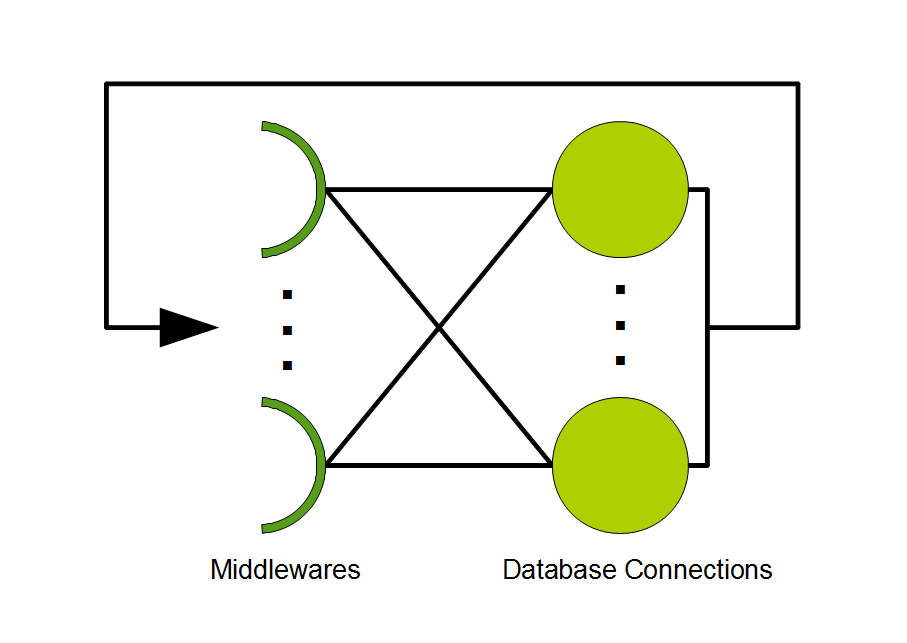
\includegraphics[width=0.9\textwidth]{globalModel}
            \caption{Simplified model of the closed queuing system for \telesto}
            \label{fig:globalModel}
    \end{figure}

\section{Workload}
    As seen in \cref{fig:globalModel}, we use a closed queuing network to model
    \telesto.

\section{Notation}

\begin{description}
\item[Arrival Process]

\end{description}

\section{Load-Dependent Service Centers}



\chapter{Performance Analysis}


\chapter{Comparison}


\chapter{Conclusion}
	

% This displays the bibliography for all cited external documents. All references have to be defined in the file references.bib and can then be cited from within this document.
\bibliographystyle{splncs}
\bibliography{references}

% This creates an appendix chapter, comment if not needed.
%\appendix
%\chapter{Appendix Chapter}

%\section{Database Structure}

	
\end{document}